Interaction between human and complex cyber-physical systems is an essential aspect of modern computing platforms. These interactions enable users to provide inputs to software systems and services and interpret computation output. Over the last half a century, researchers in academia and industry spent a significant effort to make this interaction as effortless as possible. Input-output (IO) peripherals and complex user interfaces (UI) are keys to facilitate this interaction. Such intuitive UIs were quintessential to the widespread deployment of computing devices around us and the rapid adoption of remote applications and services. 

Security and safety-critical remote applications such as e-voting, online banking, industrial control systems (such as remote PLCs~\cite{controlbyweb}), and medical devices~\cite{medicalDevice} rely upon user interaction. This is typically performed through a \emph{host} system that generally is a standard $x86$, which gives the host access to the raw IO data that is exchanged between the user and the remote server. The host consists of large and complex system software such as the operating system, device drivers, applications such as a browser, and a diverse set of hardware components that expose the host to a large attack surface. Due to cost and convenience, general-purpose PCs are prevalent in many safety-critical application domains such as industrial plants and hospitals. For example, the WannaCry ransomware incident showed that NHS hospitals relied on Windows XP platforms~\cite{berry_2017,field_wannacry_2018}. 


\begin{figure}[t]
  \centering
    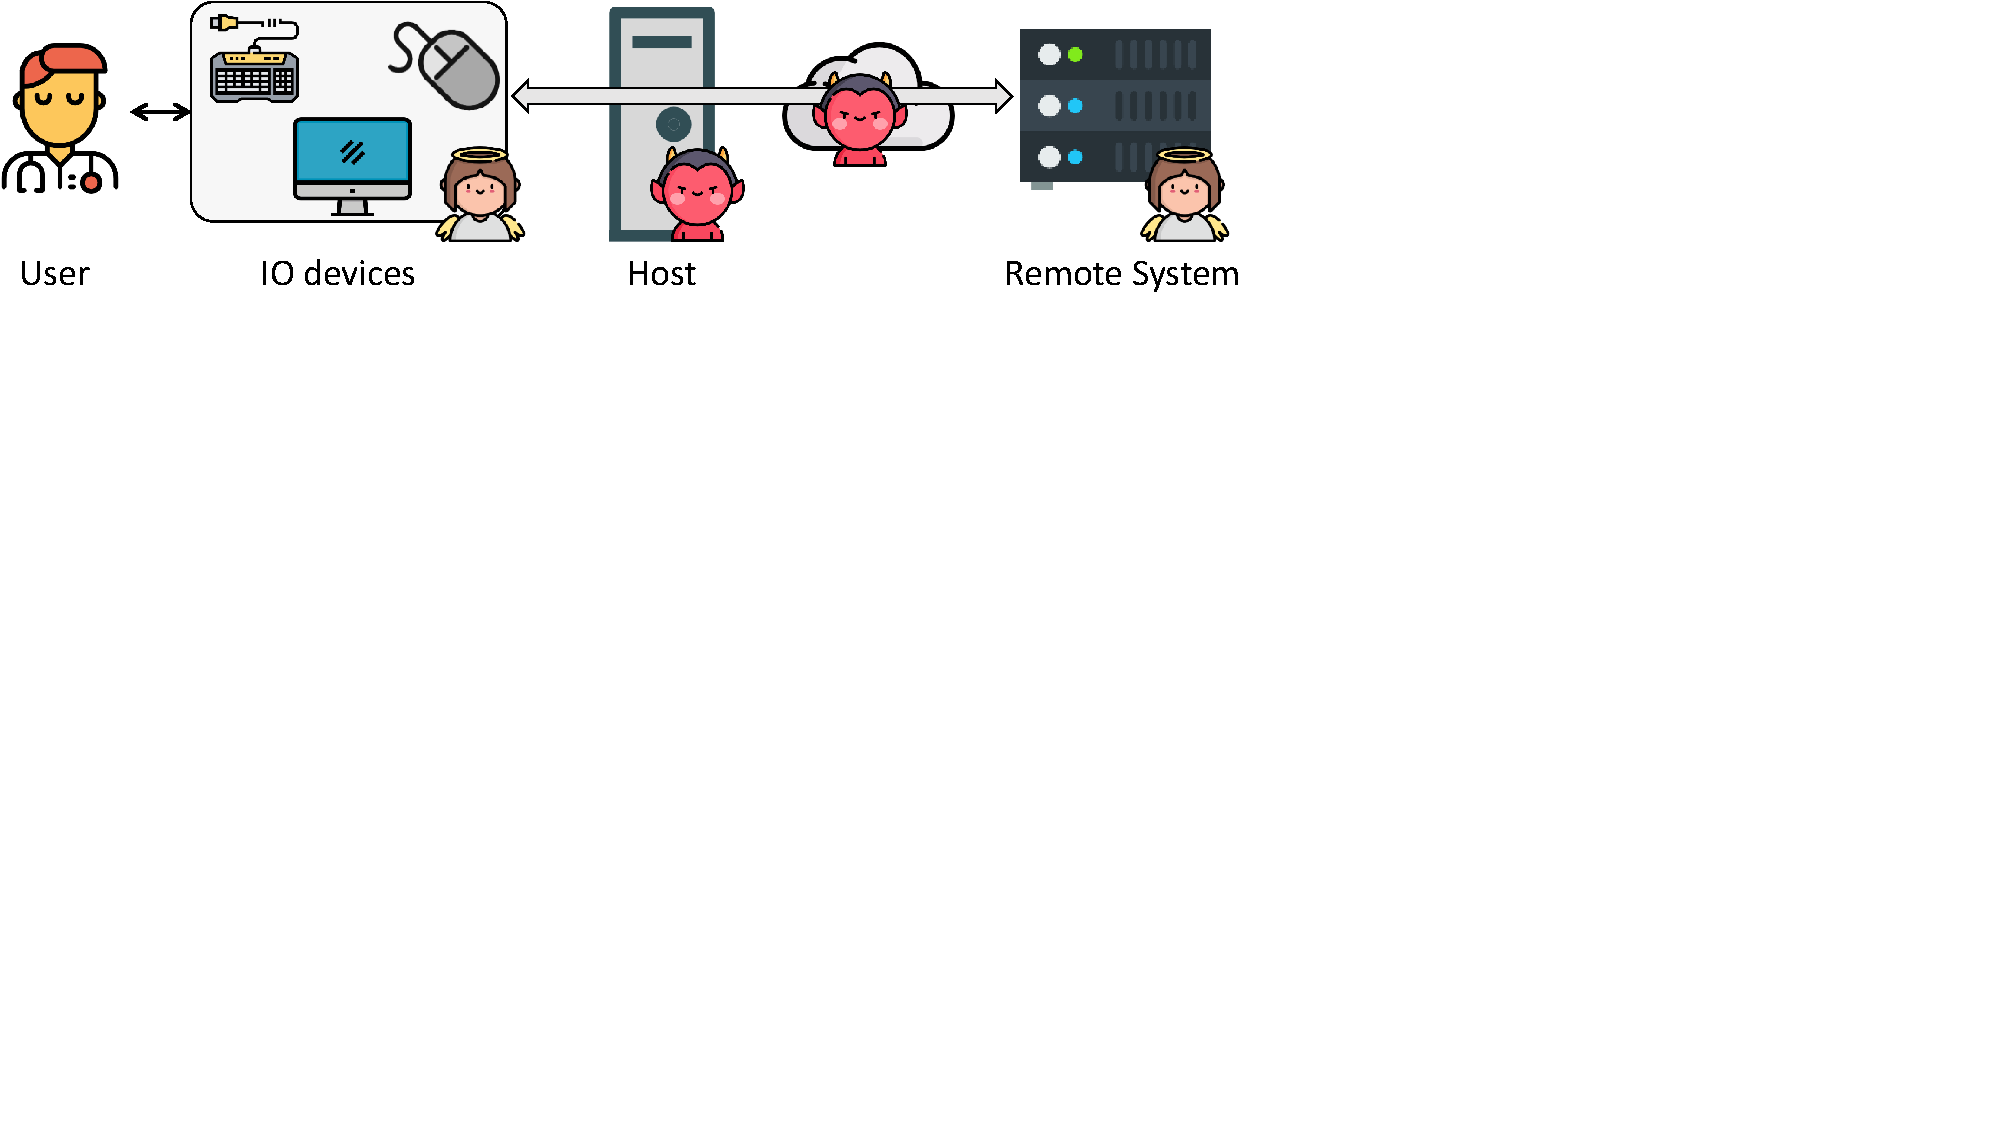
\includegraphics[trim={0 14cm 12cm 0},clip,width=\linewidth]{chapters/introduction/images/trustedPath.pdf}
    \caption[Remote trusted path through untrusted host]{\textbf{Remote trusted path through untrusted host.} }
    \label{fig:trustedPath}
\end{figure}

\section{Trusted Path Background}

\emph{Trusted path} provides a secure channel between the user (specifically through the human interface devices - HIDs) and the end-point, typically a trustworthy application running on the host. A trusted path ensures that user inputs reach the intended application unmodified, and all the outputs presented to the user are generated by the legitimate application. In certain scenarios, the trusted path also provides confidentiality of the user data. The trusted path can also be extended to general peripherals such as accelerators, GPUs, and sensors, and even remote systems. An attacker who exploits the software stack, i.e., the hypervisor or the OS and/or the hardware (refer to Figure~\ref{fig:trustedPath}), can control the user's computer. Such an attacker can \emph{observe} and \emph{modify} any user interaction data without being detected by the user or the server, hence undermining the trusted path's properties. 

The trusted path to the local host is a well-researched area where many solutions focus on using trusted software components such as a trusted hypervisor~\cite{zhou2012building} or external trusted hardware~\cite{filyanov2011uni,weigold2011secure,McCPerRei2006,mannan2007using,Fidelius}. However, hypervisors are hard to deploy, have a large TCB, and are impractical in real-world scenarios as most of the existing verified hypervisors offer a minimal set of features, and some of the external device-based approaches suffer from poor usability, security issues due to user habituation and are only limited to simple inputs.


\section{TEEs in Trusted Path}

Trusted execution environments (TEEs) drastically reduce the trusted computing base (TCB) and provide security to applications, known as enclaves, without having to trust the operating system and hypervisor~\cite{costan2016intel,winter2008trusted,costan2016sanctum}. Thus, the attack surface is reduced by eliminating two of the largest sources of vulnerabilities for a system~\cite{checkoway2013iago,suzaki2011memory}. TEEs use isolation primitives provided by the CPU to exclude all software, but a single target application (commonly known as the enclaves) from the software trusted computing base (TCB). Only the CPU is part of the hardware TCB, while the remaining hardware in the system is considered malicious. Even memory is not included in the TCB and can only be used in conjunction with memory encryption and integrity protection. Such a trust model makes the TEEs ideal candidates for the aforementioned trusted path applications where the software stack is attacker-controlled. 


While SGX's remote attestation guarantees that the attested enclave runs the expected code, it \emph{does not}, however, guarantee that the enclave runs on the expected computing platform. An adversary that controls the software stack (OS, hypervisor, etc.) on the target platform can relay incoming attestation requests to another platform. This way, the user ends up attesting to the attacker's platform rather than her own. Relay attack enables the attacker to see all the IO data to and from the user, e.g., sensitive user input on display, and execute a long-term physical side-channel attack. Hence, relay attacks on TEEs pose a real threat to the trusted path. Note that the relay attack is a long-standing open problem in trusted computing, as already a decade ago, Parno identified it in the context of TPM attestation~\cite{parno2008bootstrapping}. Hence, directly incorporating a trusted path to a TEE like Intel SGX is not a trivial issue.


Solving the relay attack still does not make TEEs ideal for a trusted path. TEEs cannot communicate with any external device without going through the malicious operating system, which is crucial for a trusted path. Hence with the current TEEs, the only way to build a trusted path is to rely on the OS or hypervisor with millions of lines of code~\cite{torvalds2020linux,barham2003xen}, results in a static hardware TCB from the enclave's perspective. This shortfall of TEEs is critical because modern, trusted path applications not only handle data for simple IO purposes but also many applications. E.g., using sensitive medical data for training machine learning models on the GPU. This new breed of applications shows a changing trend in cloud computing, known as \emph{disaggregated} computing model. Unlike the traditional CPU-centric computational model, where the CPU is the platform's sole executioner, modern data centers offload application-specific workloads to special-purpose hardware devices such as GPUs, accelerators, etc. Hence the current TEE primitives such as the isolation and the attestation need designing to support the trusted path applications in the modern disaggregated cloud data centers.   

%think about combining 1 and 2

\begin{figure}[t]
  \centering
    %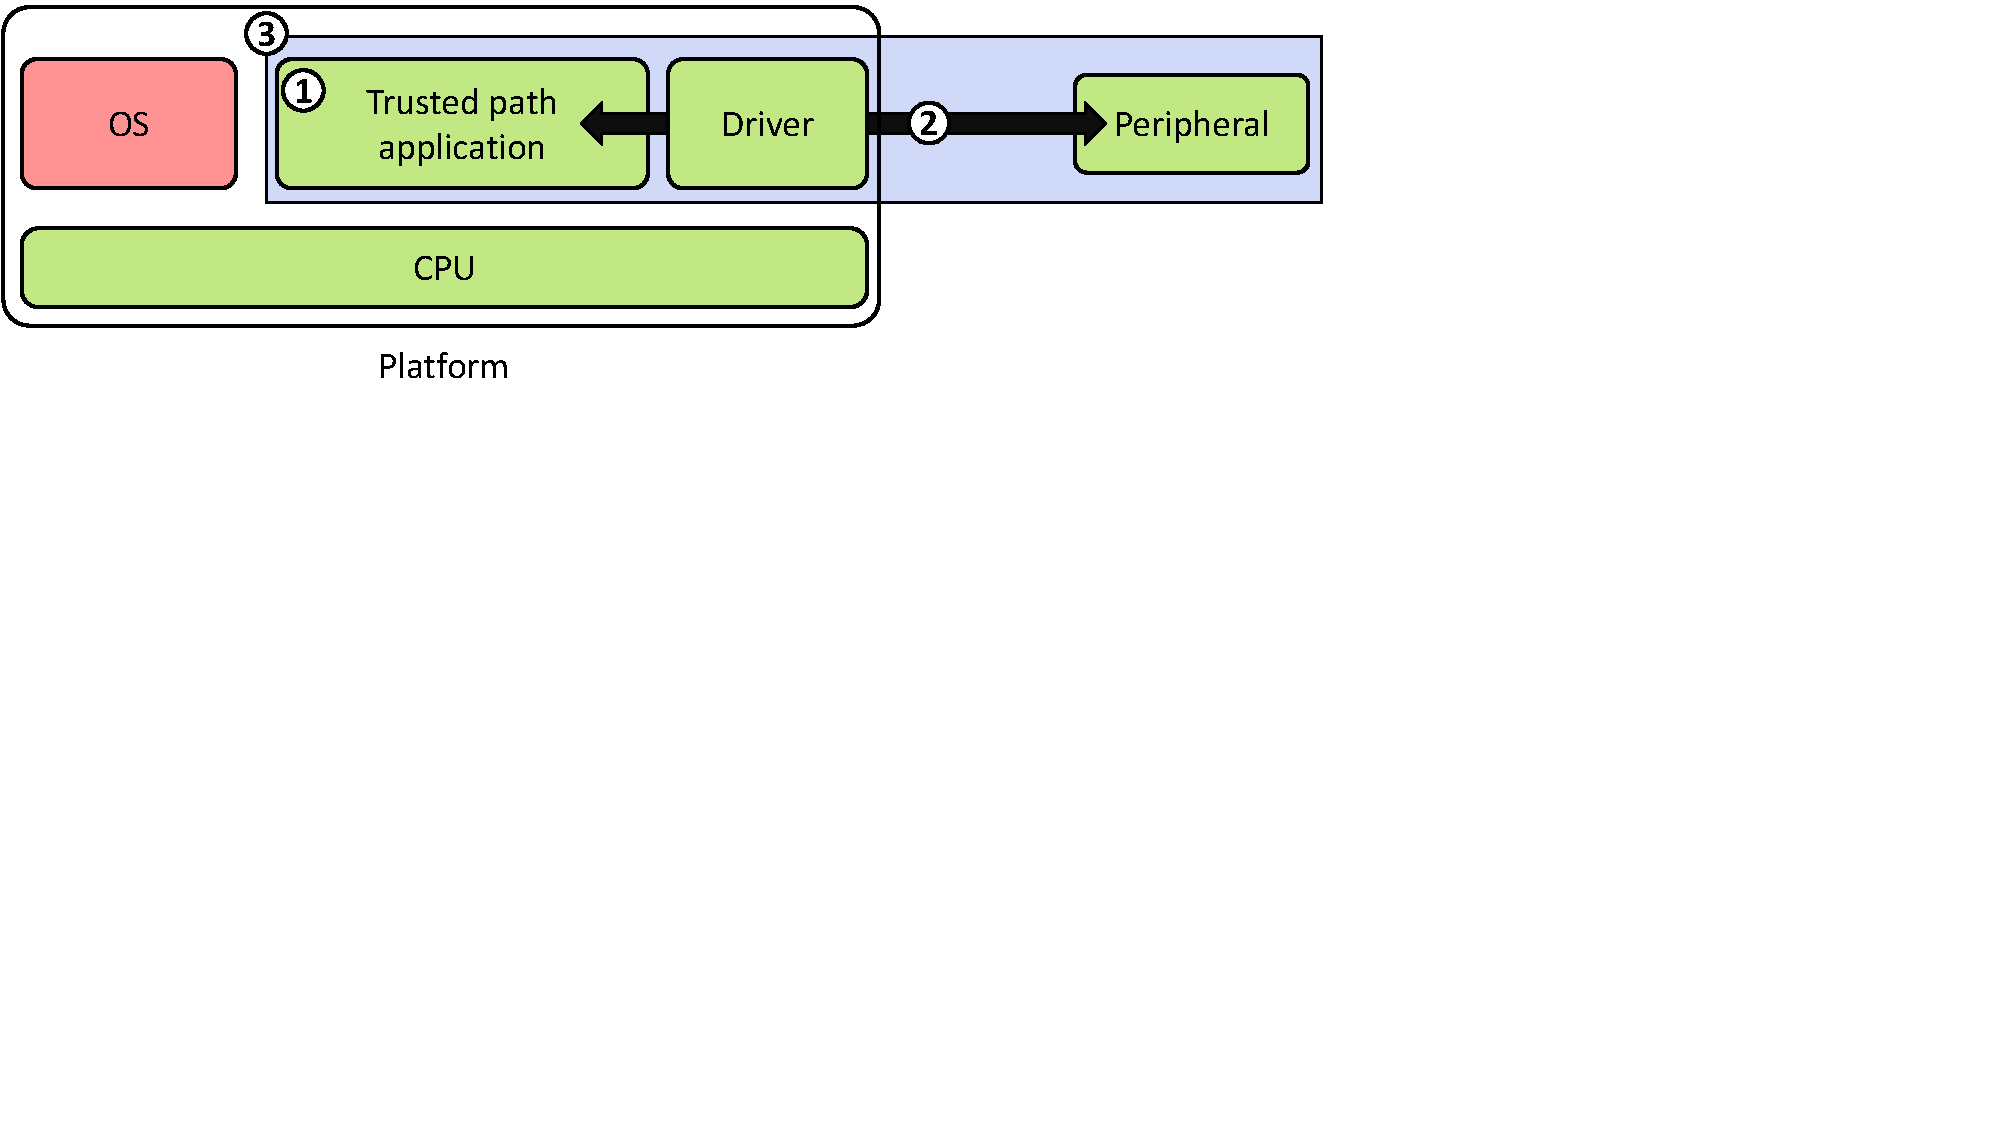
\includegraphics[trim={0 12cm 11cm 0},clip,width=\linewidth]{chapters/introduction/images/works.pdf}
    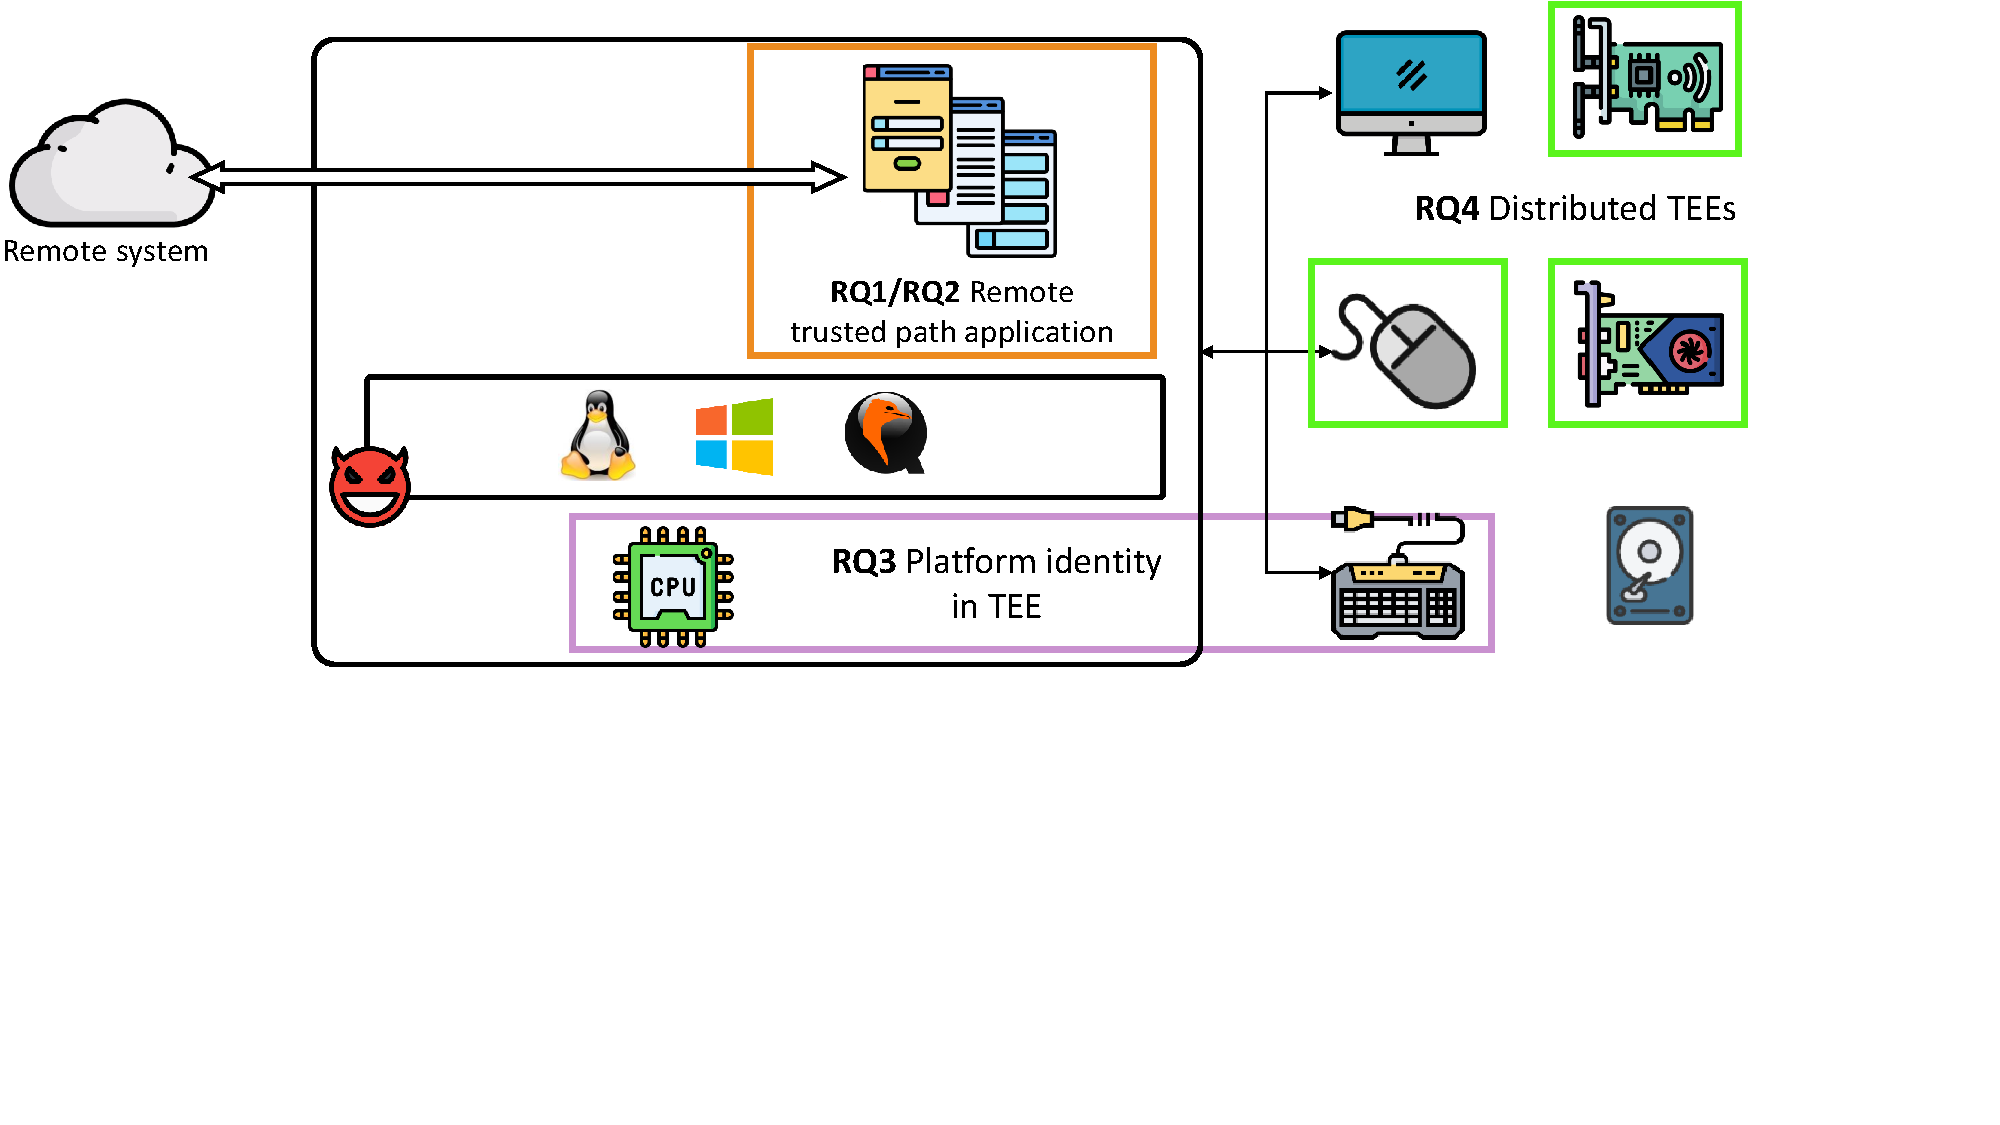
\includegraphics[trim={0 7cm 4cm 0},clip,width=\linewidth]{chapters/introduction/images/RQ.pdf}
    \caption[Research questions]{\textbf{Research question.} In this figure, we summarize the research question that we address in this thesis a context of a modern computing platform.}
    \label{fig:rq}
\end{figure}

\section{Research Questions}

Given the problem space discussed above, this thesis addresses the four following research questions (RQ) concerning the trusted path and trusted execution in modern platforms. Figure~\ref{fig:rq} depicts these research questions in the context of morn computing platforms.
\begin{enumerate}
  
  	\item[\textbf{RQ1}] How to build trusted path systems that provide integrity (and possibly confidentiality) guarantees without the users rely on cognitive-heavy solutions such as transaction confirmation devices while maintaining a small TCB? Are these systems truly provide integrity (and confidentiality property) against an attacker-controlled (both software and hardware) host?
  	
    \item[\textbf{RQ2}] Why all\footnote{to the best of our knowledge} the existing solutions failed to provide a trusted path that provides integrity and confidentiality guarantees to the user interactions? What are the fundamental security properties required for a secure trusted path in the presence of an attacker-controlled (both software and hardware) host?
    
    \item[\textbf{RQ3}] Relay attack from a local platform to a remote attacker-controlled platform is a real threat to the remote attestation of TEEs like Intel SGX. How to ensure that the attacker cannot relay the attestation to an attacker-controlled platform that exposes all the sensitive IO data?
    
    \item[\textbf{RQ4}] How to extend the trusted path mechanism to a modern platform that is interconnected with a number of heterogeneous peripheral devices? How to extend this trusted path into other complex hardware devices such as GPU or accelerator that can execute programs outside the CPU cores? How to ensure the platform-wide integrity guarantee (configuration and interaction of the TEE enclaves and external peripherals) is preserved without relying on a purpose-built system?  
\end{enumerate}


\section{Addressing the Research Question: Contribution of this Thesis}


This section provides a brief outline of the proposed solutions to address the aforementioned research questions.

\subsection{Addressing RQ1}
We propose two systems: \integrikey~\cite{integrikey} and \integriscreen~\cite{integriscreen} to answer \textbf{RQ1}, the first research question. \integrikey uses input signing to provide a second factor for the integrity of the keyboard input. In context, \integriscreen the uses a phone camera to capture the information that the user is typing on the screen to provide a second factor for user intention's integrity. Unlike exiting trusted path solutions, these proposals rely neither on transaction confirmation devices that put a heavy cognitive load on the user nor on a hypervisor or trusted drivers that introduce a large TCB. Moreover, \integriscreen provides a restricted form of output integrity to ensure that the attacker-controlled host does not manipulate UIs. \integrikey uses a small embedded trusted device that runs a few hundred LoC to sign user input. In \integrikey, we identify a new form of input manipulation attack that we name field swapping attack. In a swapping attack, the attacker can swap the levels of different input fields that accept overlapping values (e.g., blood pressure and heart rate for a medical implant). \integrikey analyzes the type of input fields, and based on the regular expression of these fields; it can compute the overlapping fields that could be vulnerable to swapping attack and recommend the user to append a label with the input value to distinguish it. 
In comparison, the \integriscreen uses a phone to verify the user input by using text recognition and send that result to the server on a different communication channel. The attacker model in \integrikey and \integriscreen differs as the latter requires trust on the smartphone for the host screen analysis. Even though both \integrikey and \integriscreen provide a significant improvement over state-of-the-art trusted path solutions, they suffer similar security and functionality pitfalls as their counterparts. They are all ad-hoc approaches focus on solving a single problem and a single input source. This leads to multiple sophisticated attacks on them (e.g., character addition/reduction attack, early form submission attack, etc.).


\subsection{Addressing RQ2}
The shortcomings of the existing literature provide the groundwork of our system named \protection that answers the first research question \textbf{RQ2}. Here we assume that the entire host (both software stack and the hardware) is attacker-controlled. We also do not assume that host has a TEE-enabled processor. \protection is built on the following observations: i) input integrity is possible only when both input and output integrity are ensured simultaneously, ii) all the input modalities are needed to be protected as they influence each other, and iii) high cognitive load results in user habituation errors. \protection uses a trusted low-TCB auxiliary device that we call \deviceprotection, which works as a mediator between all user IO devices and the untrusted host. Instead of implementing a separate network interface, the \deviceprotection uses the host as an untrusted transport - reducing the attack surface. \protection ensures output integrity and confidentiality by sending an encoded UI to the host that only the \deviceprotection can overlay on the part of the screen. The overlay is possible as the \deviceprotection intercepts the display signal between the host and the monitor. The overlay generated by the \deviceprotection ensures that the host cannot manipulate any output information on that overlaid part of the screen; hence, it can not trick the user. All the user interaction to this protected overlay is encrypted and signed by the \deviceprotection. Therefore input integrity and confidentiality are preserved.

\subsection{Addressing RQ3}

While addressing RQ2 provides the necessary mechanisms to construct a remote trusted path application, porting the same trusted path application into a trusted execution environment (TEE) such as the Intel SGX is still non-trivial due to the relay attack on the SGX's remote attestation. Parno~\cite{parno2008bootstrapping} identified distance bounding as a candidate solution to TPM relay attacks already ten years ago but concluded that it could not be realized securely as the slow TPM identification operations (signatures) make a local and relayed attestation indistinguishable. However, the implication of the relay attack was never well-studied. In this dissertation, we investigate the implication of the relay attack and show that it could have an adverse consequence. To answer the third research question, \textbf{RQ3},  We propose a new solution, called \proximitee, that prevents relay attacks by leveraging a simple embedded device that we call \deviceproximitee that is attached to the attested target platform. The \deviceproximitee executes a challenge-response protocol between itself and the platform and based on the latency of the protocol, and the \deviceproximitee determines if it is connected to the target platform physically or not. In short, \deviceproximitee leverages distance bounding protocol to estimate the physical closeness to the target platform. Our solution is best suited (but not limited to) to scenarios where i) the deployment cost of such an embedded device is minor compared to the benefit of more secure attestation, ii) trust-on-first use (ToFU) solutions are not acceptable, and iii) most importantly, in data center scenario, simply plugging in or out the \deviceproximitee allocate or revoke a specific platform from a data center fleet without explicitly relying on a public key ledger. Attestation of servers at cloud computing platforms and setup of SGX-based permissioned blockchains are two such examples. Note that, in contrast to the earlier research questions (RQ1 and RQ2), we only assume that the software stack and the network is fully attacker-controlled and the CPU to be trusted.


\subsection{Addressing RQ4}
Finally, to answer \textbf{RQ4}, the last research question, We propose a TEE with a \emph{configurable} software and hardware TCB including arbitrary external peripheral devices, a concept that we name \emph{platform isolation environment} (\pie). \pie executes applications in \emph{platform-wide enclaves}, which are analogous to the enclaves provided by TEEs, except that they span several hardware components. For example, a \nameenclave{} can be composed of an output device such as a display, input devices such as keyboard and mouse, the CPU that is executing the program, the GPU that renders the graphics, and the custom code running on them. Like in traditional enclaves, a \nameenclave{} can be remotely attested. However, the \pie attestation not only reports a measurement of the software TCB but also of the hardware components that are part of the \nameenclave{}.


The shift towards configurable hardware and software TCBs has wide-ranging implications concerning integrity, confidentiality, and attestation of a \nameenclave{}. 
Attestation, for one, should cover all individual components of a \nameenclave{} atomically to defend against an attacker that changes the configuration in between attestations to separate components. 
Moreover, the untrusted OS may remap the peripheral devices at runtime with an untrustworthy device, which should not receive access to sensitive data. We carefully design \pie to not be vulnerable to such attacks and present an in-depth security analysis.

We mitigate the above-mentioned attacks with two new properties of \nameenclave{}s: \emph{platform-wide attestation} and \emph{platform awareness}. Platform-wide attestation expands the attestation to cover all components within a \nameenclave, and platform awareness enables enclaves to react to changes in their ecosystem, i.e., remapping by the OS.
We achieve this by introducing two new events into the enclave lifecycle, \textit{connect} and \textit{disconnect}, which allow to track the liveliness of one enclave from another.


\begin{figure}[t]
  \centering
    %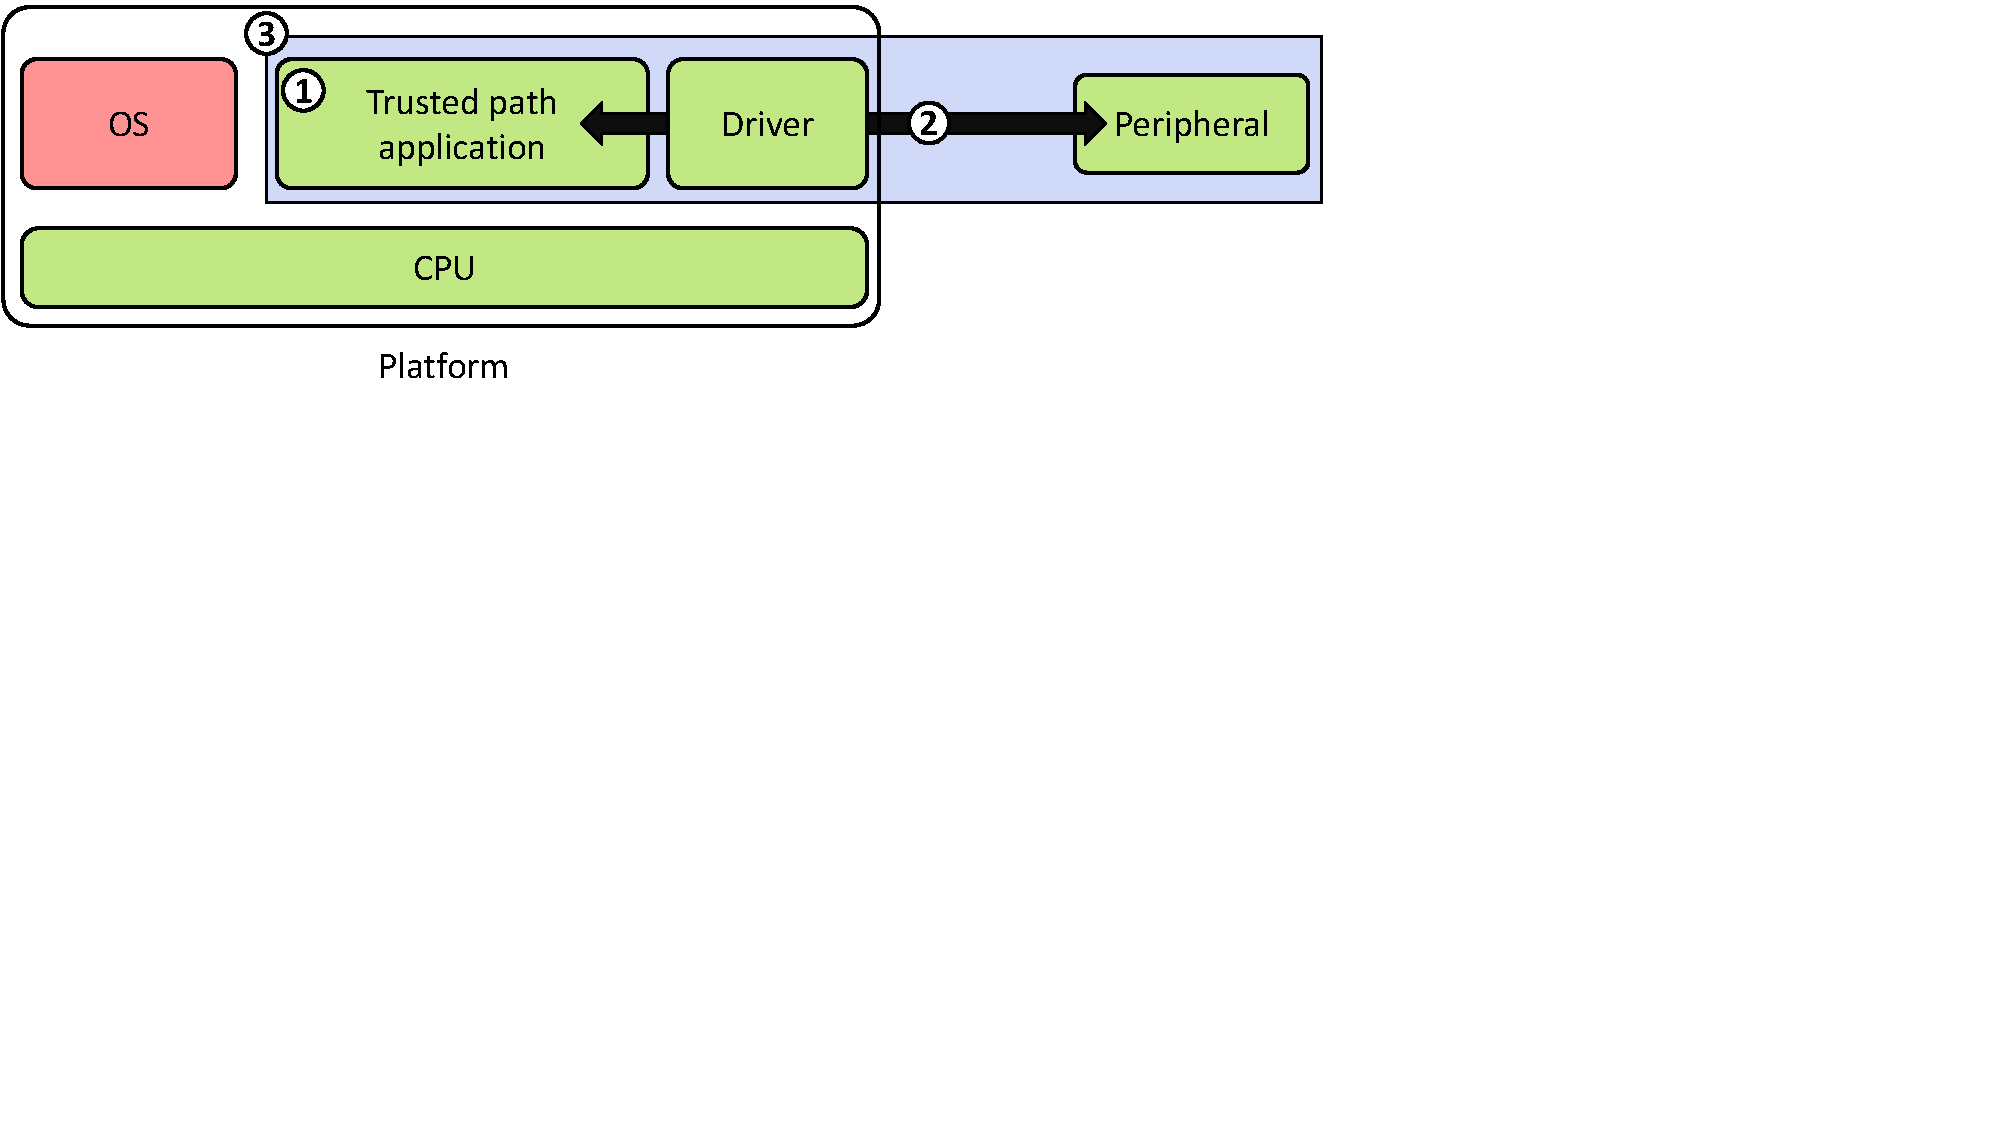
\includegraphics[trim={0 12cm 11cm 0},clip,width=\linewidth]{chapters/introduction/images/works.pdf}
    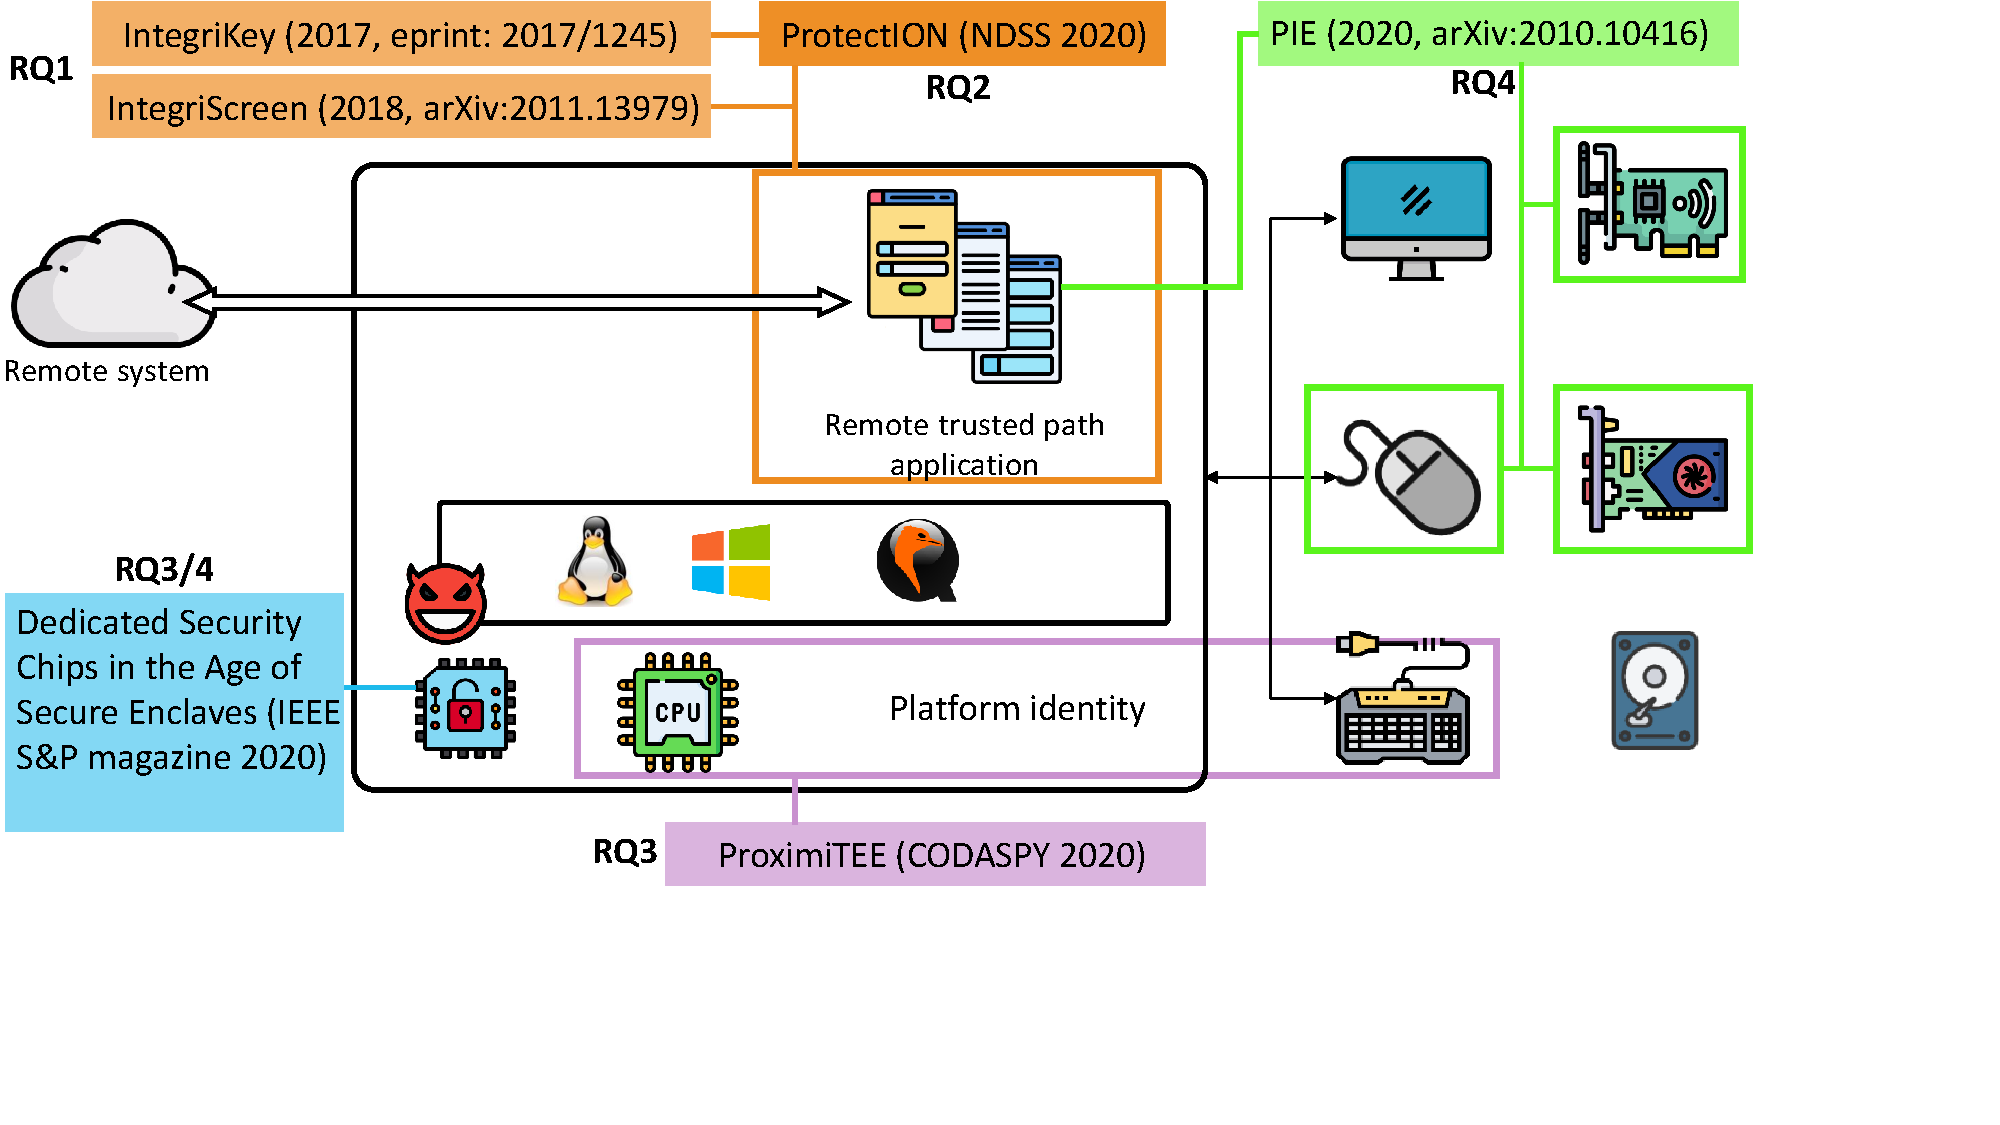
\includegraphics[trim={0 3cm 4cm 0},clip,width=\linewidth]{chapters/introduction/images/works_1.pdf}
    \caption[Summary of the works in this thesis]{\textbf{Summary of the works in this thesis.} In this figure, we summarize the works that are in the thesis in a context of a modern computing platform.}
    \label{fig:works}
\end{figure}

In summary, Figure~\ref{fig:works} provides an overview of all the works included in this thesis.

\section{Summary of the Contributions and Organization}

The contributions of this thesis are divided into four parts and summarized as the following:

\begin{enumerate}[leftmargin=*]
  
  \item[] \textbf{Part 1: How (not) to build a trusted path: providing negative results on how system-oriented way of proposing trusted path solution can lead to insecure systems.}
  
  \begin{itemize}
  \item Chapter~\ref{ch:integrikey}: \integrikey, an input signing approach to provide the second factor for integrity in user input through input signing
  %\footnote{Note that this work presents negative results and shows how an input signing method is not secure. However, the chapter also explores a new input manipulation attack - label swapping attack,}

\begin{enumerate}
    \item \emph{New attack.} In \integrikey, we identify swapping attacks as a novel form of user input manipulation against simple user input matching strategies.
    \item \integrikey. We design and implement a user input integrity protection system that is tailored for keyboard input, prevents swapping attacks, and is easy to deploy.
    \item \integrikey{} tool. We develop a user interface analysis and webpage annotation tool that helps developers to protect their web services and minimizes user effort. However, later analysis shows that the input signing is insecure. This is not due to the implementation of the input signing method, rather the fundamental pitfall of the method.
    \item \emph{Evaluation.} We verified that our tool could process UIs of existing safety-critical systems and cryptocurrency wallets correctly. Our experiments show that the performance delay of \integrikey user input integrity protection is low. Our preliminary user study indicates that user input labeling prevents swapping attacks in most cases.
   %, and our preliminary user study indicates that users can perform the needed labeling.
\end{enumerate}

	\item Chapter~\ref{ch:integriscreen}: \integriscreen, second factor for user intention integrity through UI analysis captured through a smartphone\footnote{\integriscreen was a collaboration between multiple researchers. This thesis only includes my primary contribution in \integriscreen: the development of \integriscreen{}'s main idea, security analysis, and implementation of the \integriscreen{}s server-side component.}.

\begin{enumerate}
\item \textbf{Novel approach for transaction confirmation.} We design \integriscreen based on \emph{screen supervision}, which differs fundamentally from the existing alternatives, integrates well with user devices (e.g., smartphones), and has the potential to offer high integrity guarantees for the user inputs in the presence of compromised hosts.

\item \textbf{Prototype implementation and evaluation.} We implement a prototype dubbed \integriscreen as an Android app and server-side component. Moreover, we perform a variety of experiments, which show the system is practical, effective, and performs well. 

\item \textbf{Future challenges.} We are the first to explore the use of \emph{screen supervision} for security, and especially in the context of transaction confirmation solutions. This new paradigm opens new possibilities for continuous supervision of user inputs over the limitations of existing solutions while neither risking user habituation nor increasing their efforts.
\end{enumerate}

\end{itemize}


\item[] \textbf{Part 2: Fundamental security properties for trusted path, attacks on existing systems and building new systems that incorporate these fundamental security properties.}

\begin{itemize}
    \item Chapter~\ref{ch:protectIOn}: \protection: Root-of-Trust for IO in Compromised Platforms
    \begin{enumerate}
      
      	\item \textbf{Identification of new attacks:} We identify two new attacks on the existing trusted path systems. The first one is \emph{input addition/reduction} attack on trusted path systems that uses input signing. \integrikey is susceptible to this attack. Another attack is \emph{early form submission} attack that targets target path systems that do not consider all modalities of input.
      	 
        \item  \textbf{Identification of IO security requirements:} We identify new requirements for trusted path based on the drawbacks of the existing literature: i) unless both output and input integrity are secured simultaneously, it is impossible to achieve any of the two, and ii) without protecting the integrity of all the modalities of inputs, none could be achieved.
        
        \item \textbf{System for IO integrity:} We describe the design of \protection, a system that provides a remote trusted path from the server to the user in an attacker-controlled environment. The design of \protection leverages a small, low-TCB auxiliary device that acts as a \emph{root-of-trust} for the IO. \protection ensures the integrity of the UI, specifically the integrity of mouse pointer and keyboard input. \protection is further designed to avoid user habituation.
        
        \item \textbf{System for IO confidentiality:} We also describe an extension of \protection that provides IO confidentiality, where the user needs to execute an operation like a secure attention sequence (SAS) to identify the trusted overlay on display.
        
        \item \textbf{Implementation and evaluation:} We also implement a prototype of \protection and evaluate its performance ).
    \end{enumerate}

\end{itemize}
   
   
\item[] \textbf{Part 3: Understanding relay attack in the context of Intel SGX remote attestation considering a secure trusted path enclave.}

\begin{itemize}
    \item Chapter~\ref{ch:proximitee}: \proximitee: Understanding Relay attacks on in Intel SGX remote attestation and building system for addressing the relay attacks in different attacker models (non-emulating vs. emulating attacker).
    
    \begin{enumerate}
        \item \textbf{Analysis of relay attacks.} While relay attacks have been known for more than a decade, their implications have not been fully analyzed. We provide the first such analysis and show how relaying amplifies the adversary's capabilities for attacking SGX enclaves.   

        \item \textbf{\proximitee, a system for addressing relay attacks.} We propose a hardened SGX attestation mechanism based on an embedded device and proximity verification to prevent relay attacks. \proximitee does not rely on the common trust on first use (ToFU) assumption, and hence, our solution improves the security of previous attestation approaches. Note that the distance bounding approaches are well-known in the literature, but using such a method in the context of SGX is non-trivial.
    
        \item \textbf{Experimental evaluation.} We implement a complete prototype of \proximitee and evaluate it against a very strong and fast adversary. Our evaluation is the first to show that proximity verification can be both secure and reliable for TEEs like SGX.
    
        \item \textbf{Addressing emulation attacks.} We also propose another attestation mechanism based on boot-time initialization to prevent emulation attacks. This mechanism is a novel variant of TOFU with deployment, security, and revocation benefits.
    \end{enumerate}
\end{itemize}   

\item[] \textbf{Part 3: Generalizing platform security in the context of TEEs and peripherals}
    
  \begin{itemize}  
    \item Chapter~\ref{ch:pie}: \pie:A Platform-wide TEE
    
    \begin{enumerate}
        \item \textbf{Security properties for platform-wide integrity} We extend traditional TEEs by introducing a dynamic hardware TCB. We call these new systems platform isolation environment (\pie{}). We identify key security properties for \pie{}, namely \emph{platform-wide attestation} and \emph{platform awareness}.
        template
        \item \textbf{Programming model} We propose a programming model that provides flexibility to the developers is comparable to the modern operating systems for developing enclaves that communicate with peripherals. The programming model abstracts the underlying hardware layer. 
        
        \item \textbf{Prototype and experimental evaluation} We demonstrate a prototype of a \pie{} based on Keystone~\cite{keystone} on an open-source RISC-V processor~\cite{ariane}. The prototype includes a simplified model of the entire platform, including external peripherals emulated by multiple Arduino microcontrollers. In total, our modifications to the software TCB of Keystone only amount to around 350 LoC.

    \end{enumerate}
	\end{itemize}
\end{enumerate}

\iffalse
\section{Thesis Organization}

The thesis is organized in three parts and 6 chapters (including introduction). Part 1 consists of Chapter~\ref{ch:integrikey} and~\ref{ch:integriscreen} that provide details of the two ad-hoc trusted path systems based on two different second-factor methods:\integrikey and \integriscreen. \integrikey is based on input signing, and \integriscreen is based on the visual verification of user intent. In Part 2, Chapter~\ref{ch:protectIOn}, we discussed \protection that explores fundamental security properties of the remote trusted path and shows attacks on existing trusted path solutions. Next, in Chapter~\ref{ch:proximitee}, we discuss the challenges with relay attacks when we try to port an existing trusted path application to a TEE like Intel SGX, and we address this by introducing a new system based on distance-bounding mechanism: \proximitee. \proximitee shows how one can compromise a trusted path application without even compromising any security properties of the trusted path itself, but only by compromising underlying TEE properties - remote attestation. Chapter~\ref{ch:pie} in Part 3 describes \pie, where we address the new challenges that arise from the disaggregated computing model where the trusted path application is not only bounded to the CPU cores, rather distributed among different hardware components of the platform such as a GPU, TPU, NIC, etc. Finally, Chapter~\ref{ch:summary} provides summary and concluding remarks.
\fi


\section{Publications}

Parts of this thesis are based on the following articles I have co-authored.

\begin{itemize}
  
  \item \textbf{Aritra Dhar}, Enis Ulqinaku,Kari Kostiainen, and Srdjan Capkun, ProtectIOn: Root-of-Trust for IO in Compromised Platforms, \emph{In Proceedings of the 27th Annual Network and Distributed System Security Symposium, NDSS 2020}. 
  
  \item \textbf{Aritra Dhar}, Ivan Puddu, Kari Kostiainen, and Srdjan Capkun, ProximiTEE: Hardened SGX Attestation by Proximity Verification, \emph{In Proceedings of the Tenth ACM Conference on Data and Application Security and Privacy (CODASPY '20)}. (\faTrophy)
  
  \item Moritz Schneider*, \textbf{Aritra Dhar}*, Ivan Puddu, Kari Kostiainen, and Srdjan Capkun, PIE: A Dynamic TCB for Remote Systems with a Platform Isolation Environment, \emph{arXiv preprint /2010.10416 (2020)} (*shared first authorship).
  
  \item Kari Kostiainen, \textbf{Aritra Dhar}, and Srdjan Capkun, Dedicated Security Chips in the Age of Secure Enclaves, in \emph{IEEE Security \& Privacy, vol. 18, no. 5, pp. 38-46, Sept.-Oct. 2020}.
  
  \item Ivo Sluganovic, Enis Ulqinaku, \textbf{Aritra Dhar}, Daniele Lain, Srdjan Capkun, and Ivan Martinovic, IntegriScreen: Visually Supervising Remote User Interactions on Compromised Clients, \emph{arXiv preprint 2011.13979 (2020)}.
   
  \item \textbf{Aritra Dhar}, Der-Yeuan Yu, Kari Kostiainen, and Srdjan Capkun, IntegriKey: End-to-End Integrity Protection of User Input, \emph{IACR Cryptology ePrint Archive 2017: 1245 (2017)}.
 
\end{itemize}

 In addition, during my Ph.D., I co-authored the following publications that are non included in this thesis.
 
 \begin{itemize}
   \item Vasilios Mavroudis, Karl Wust, \textbf{Aritra Dhar}, and Kari Kostiainen, Srdjan Capkun:, Snappy: Fast On-chain Payments with Practical Collaterals, \emph{In Proceedings of the 27th Annual Network and Distributed System Security Symposium, NDSS 2020}. 
   \item David M. Sommer, \textbf{Aritra Dhar}, Luka Malisa, Esfandiar Mohammadi, Daniel Ronzani, and Srdjan Capkun, Deniable Upload and Download via Passive Participation, \emph{In Proceedings of the 16th USENIX Symposium on Networked Systems Design and Implementation, NSDI 2019}.
   \item Garvita Allabadi, \textbf{Aritra Dhar}, Ambreen Bashir, Rahul Purandare, METIS: Resource and Context-Aware Monitoring of Finite State Properties, \emph{In Proceedings of International Conference on Runtime Verification, RV 2018}. (\faTrophy)
   \item Sinisa Matetic, Mansoor Ahmed, Kari Kostiainen, \textbf{Aritra Dhar}, David M. Sommer, Arthur Gervais, Ari Juels, and Srdjan Capkun, ROTE: Rollback Protection for Trusted Execution, \emph{In Proceedings of the USENIX Security Symposium 2017}.
 \end{itemize}